% =====================================================================
%  SLAPBench -- Supplementary Material
%  ECCV 2026 FoundGen-Bio workshop.  Submitted as a SEPARATE file from the
%  main paper (it is not an appendix).  Compile the same way as main.tex.
%  TODO REVIEW: put your OpenReview submission ID in ID=*****
% =====================================================================
\documentclass[runningheads]{llncs}

\usepackage[review,year=2026,ID=*****]{eccv}
%\usepackage{eccv}   % <- camera-ready

\usepackage{eccvabbrv}
\usepackage{graphicx}
\usepackage{amsmath,amssymb,amsfonts}
\usepackage{booktabs}
\usepackage{xcolor}
\usepackage{float}
% \usepackage[accsupp]{axessibility}   % enable on Overleaf
\usepackage[pagebackref,breaklinks,colorlinks,citecolor=eccvblue]{hyperref}

\graphicspath{{figures/}}

% Number supplementary figures S1, S2, ...
\renewcommand{\thefigure}{S\arabic{figure}}

\begin{document}

\title{SLAPBench: Benchmarking Multimodal Large Language Models
       for Four-Finger SLAP Fingerprint Verification\\
       \large Supplementary Material}
\titlerunning{SLAPBench (Supplementary)}
\author{Bibesh Pyakurel \and M.~G.~Sarwar Murshed}
\authorrunning{B.~Pyakurel and M.~G.~S.~Murshed}
\institute{Computer Science Department,
           University of Wisconsin--Green Bay, Green Bay, WI, USA}
\maketitle

This document collects supporting figures referenced in the main paper. It
does not introduce new claims; all results it illustrates are stated and
quantified in the main text.

\begin{figure}[htbp]
  \centering
  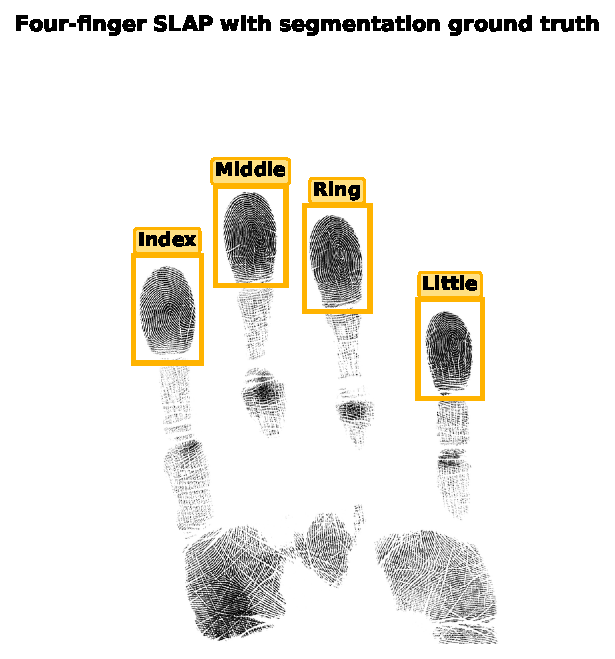
\includegraphics[width=0.55\linewidth]{fig_slap_anatomy.pdf}
  \caption{\textbf{Four-finger SLAP capture with segmentation ground truth}
    (NIST SD302b, Device~R, 500~PPI; referenced in Section~3.3 of the main
    paper). The per-finger regions (index, middle, ring, little) come from the
    segmentation coordinates distributed with SD302b. A single frame holds
    four overlapping fingers of broadly similar morphology, so any two SLAP
    images look globally alike whether they are mated or not, which underlies
    the positive-bias collapse analyzed in the main paper.}
  \label{fig:supp_anatomy}
\end{figure}

\begin{figure}[htbp]
  \centering
  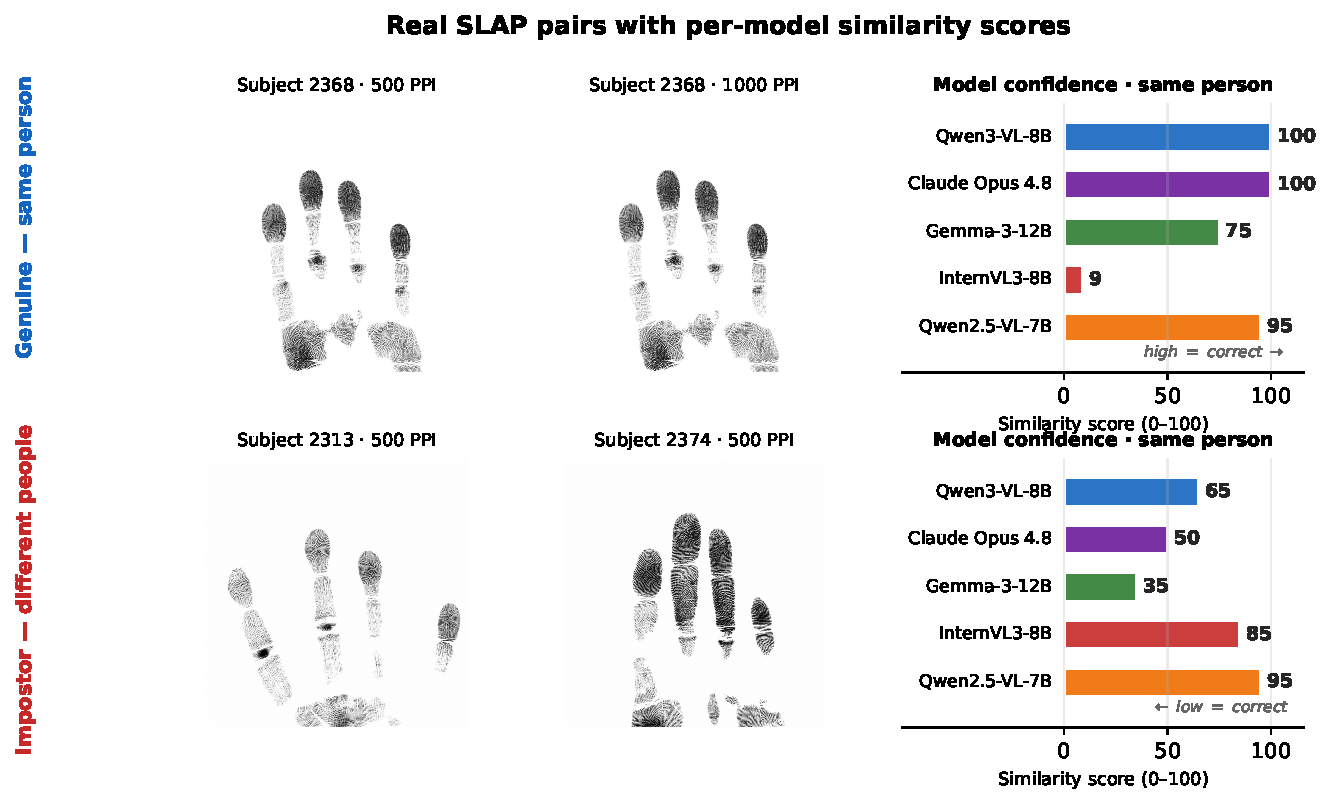
\includegraphics[width=0.9\linewidth]{fig_qualitative.pdf}
  \caption{\textbf{Real SLAP pairs with each model's similarity score
    (0--100)}, referenced in Section~5.2 of the main paper.
    \textbf{Top:} a mated pair (subject~2368, 500 vs.\ 1000~PPI); every model
    but InternVL3-8B reports high confidence, while InternVL3 inverts and
    returns~9. \textbf{Bottom:} a non-mated pair (subjects~2313 and~2374);
    Qwen3-VL-8B, Claude, and Gemma assign lower confidence, whereas
    InternVL3-8B~(85, inverted) and Qwen2.5-VL-7B~(95, saturated) falsely
    accept it. The italic cue marks which direction is correct for each pair.}
  \label{fig:supp_qualitative}
\end{figure}

\begin{figure}[htbp]
  \centering
  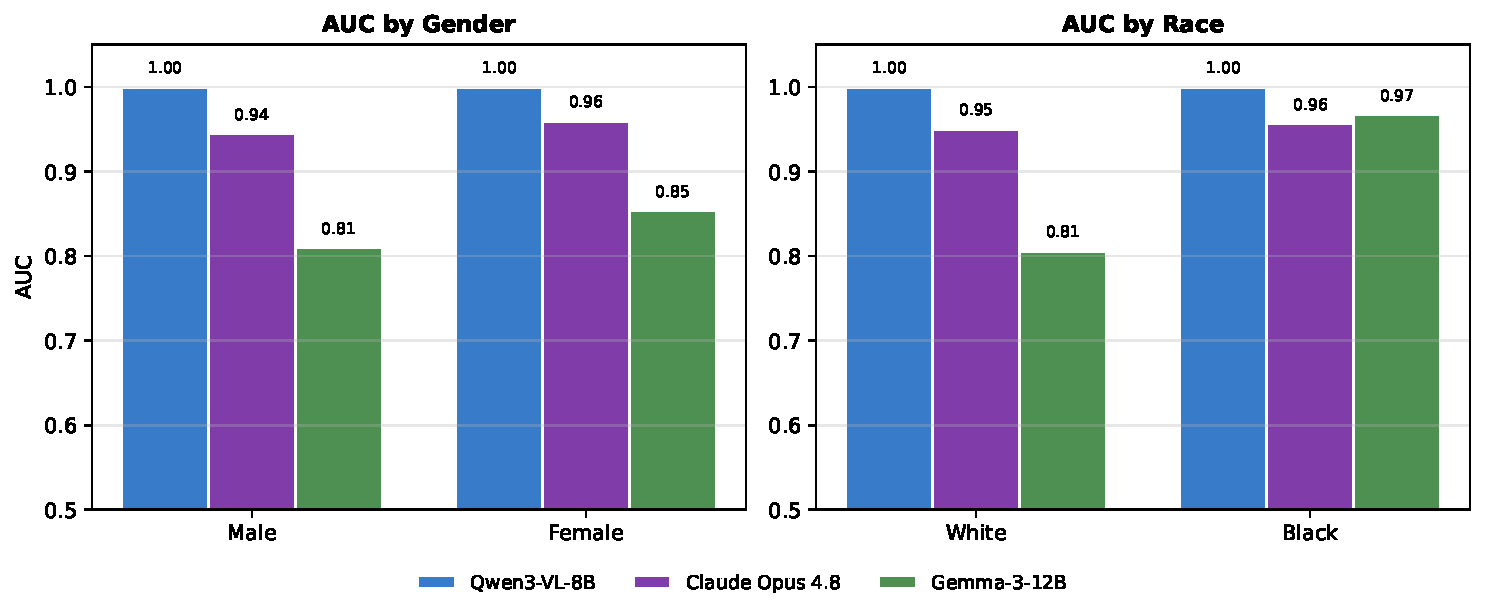
\includegraphics[width=0.85\linewidth]{fig_fairness.pdf}
  \caption{\textbf{Per-subgroup AUC by gender and race} for the three
    discriminating models, referenced in Section~5.4 of the main paper (the
    numeric values appear in Table~2 there). Qwen3-VL-8B is uniformly perfect;
    Claude Opus~4.8 shows small gaps ($\leq$1.5~AUC points by gender);
    Gemma-3-12B shows the largest disparities. The Black race group is small
    ($n_i = 272$), so Gemma's high value there should be read with caution.}
  \label{fig:supp_fairness}
\end{figure}

\begin{figure}[htbp]
\centering
\footnotesize
\setlength{\fboxsep}{6pt}
\noindent\fbox{\parbox{0.95\linewidth}{%
\textbf{System prompt (all strategies).}\enspace
{\ttfamily You are an expert fingerprint examiner.}
\vspace{4pt}\hrule\vspace{4pt}
\textbf{Zero-shot (ZS).}\\
{\ttfamily Below are two SLAP fingerprint images. A SLAP image captures four
fingers from one hand pressed simultaneously on a scanner.\\
Do these two images belong to the same person?\\
(A) Yes, same person\quad(B) No, different people\\
Reply with only the letter A or B.}
\vspace{4pt}\hrule\vspace{4pt}
\textbf{Task description (TD).}\\
{\ttfamily A SLAP fingerprint image captures four fingers from one hand
simultaneously. The same person's fingers produce slightly different images
each time they press the scanner (different pressure, slight movement), but
the ridge patterns remain the same. Below are two SLAP fingerprint images. Do
these two images belong to the same person?\\
(A) Yes, same person\quad(B) No, different people\\
Reply with only the letter A or B.}
\vspace{4pt}\hrule\vspace{4pt}
\textbf{Similarity scoring (SS).}\\
{\ttfamily You are a forensic fingerprint examiner analyzing two SLAP
fingerprint images. A SLAP image captures four fingers (index, middle, ring,
little) pressed simultaneously on a scanner. Your task: Examine the ridge flow
patterns, ridge endings, bifurcations, and the relative shape and spacing of
each finger across both images. Then return a single integer between 0 and 100
representing your confidence that both images belong to the same person, where
0 = certain they are different people, 50 = completely uncertain, and
100 = certain they are the same person. A score of 65 means you are 65\%
confident the images are from the same person. Reply with the number only. Do
not include any text, explanation, or label.}
}}
\caption{The three prompt templates, reproduced verbatim (referenced in
  Section~4.3 of the main paper). Every model receives the same system prompt
  and, per strategy, the same user prompt, with the two SLAP images attached to
  the user message. \texttt{\%} denotes a literal percent sign.}
\label{fig:supp_prompts}
\end{figure}

\section{Demographic Fairness Detail}

This section gives the full protocol and per-subgroup table for the fairness
analysis summarized in Section~5.4 of the main paper. We recompute
similarity-scoring performance within demographic subgroups: a mated pair is
assigned to a subgroup by its subject's attribute, and a non-mated pair is
counted within a subgroup only when \emph{both} subjects share that attribute.
The analysis is restricted to the three discriminating models (subgroup
breakdowns of the two near-random models are uninformative) and to subgroups
with sufficient support among the 88~clean subjects (gender; White and Black
race; three age bands); Asian, ``other,'' and ``no answer'' race groups
($\leq 6$ subjects) are too small to evaluate reliably.

\begin{table}[htbp]
\centering
\caption{Per-subgroup similarity-scoring performance (AUC / EER\%) for the
  three discriminating models. $n_g$/$n_i$ are the mated and within-group
  non-mated pair counts. Small subgroups (Black, 18--30) are reported with
  caution. Qwen3-VL-8B is uniform at AUC~$= 1.000$ across all groups, which
  must be read alongside the perfect-score caveat of the main paper.}
\label{tab:supp_fairness}
\renewcommand{\arraystretch}{1.2}
\setlength{\tabcolsep}{5pt}
\begin{tabular}{l rr ccc}
\toprule
\textbf{Subgroup} & \textbf{$n_g$} & \textbf{$n_i$}
  & \textbf{Qwen3} & \textbf{Claude} & \textbf{Gemma} \\
\midrule
Male    &  70 & 1190 & 1.000 / 0.0 & 0.945 / 13.2 & 0.810 / 15.6 \\
Female  & 106 & 2756 & 1.000 / 0.0 & 0.960 / 10.5 & 0.854 / 14.8 \\
\midrule
White   & 122 & 3660 & 1.000 / 0.0 & 0.950 /  7.4 & 0.806 / 18.3 \\
Black   &  34 &  272 & 1.000 / 0.0 & 0.957 / 11.6 & 0.968 /  4.4 \\
\midrule
18--30  &  26 &  156 & 1.000 / 0.0 & 0.967 /  6.1 & 0.815 / 19.2 \\
31--45  &  76 & 1406 & 1.000 / 0.0 & 0.944 / 13.8 & 0.826 / 15.8 \\
46+     &  74 & 1332 & 1.000 / 0.0 & 0.957 / 10.6 & 0.858 / 13.5 \\
\bottomrule
\end{tabular}
\end{table}

Claude Opus~4.8 varies by at most 1.5~AUC points across gender (male 0.945,
female 0.960) and 0.7 across White/Black. Gemma-3-12B shows the widest spread,
with a 4.4-point gender gap and an EER swing from 18.3\% to 4.4\% between White
and Black; that Black subgroup rests on only 272 within-group non-mated pairs
from 17 subjects, so neither its values nor any disparity from them should be
over-read.

\end{document}
